\documentclass
[answers]
{exam}

\linespread{1.1}

\usepackage{amsmath, amssymb, amsthm}  %% 數學符號用txfonts
\usepackage{mathrsfs} 
%\usepackage{pstricks,pstricks-add} % 引入 pstricks 和 pstricks-add 套件 (繪圖套件) 
%插入GGB圖片===================================
\usepackage{pgf,tikz}
\usepackage{mathrsfs}
\usetikzlibrary{arrows}
%=============================================
\usepackage{graphicx}   %% 插入圖片用
\usepackage{float}  %%強制插入圖片位置
\usepackage{caption}
\usepackage{subfigure}
\usepackage{color}
%\usepackage{minitoc}   %chapter下的小目錄
\usepackage{colortbl}
\usepackage{nopageno}
\usepackage{cases}
\usepackage{textcomp}             % for \textcelsius
\renewcommand{\arraystretch}{1.2} % 將表格行間距加大為原來的 1.2 倍
\arrayrulewidth=1pt               % 調整線條粗細為 1pt
\tabcolsep=15pt                   % 調整欄間距為 24pt


%\begin{figure}[h]
%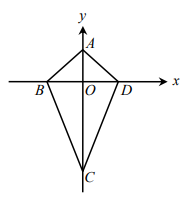
\includegraphics[scale=1.2]{./figure/2.png}
%\end{figure}

\usepackage{wrapfig}  %%圖文並排

%\begin{wrapfigure}{r}{6cm}  r:圖片靠右  6cm:離右邊6cm
%	\centering  圖片在右邊區塊的中間
%	\includegraphics[scale=0.6]{./figure/19.png}
%\end{wrapfigure}

\usepackage{tcolorbox}  %% 顏色方框
\usepackage{tikz}  %%繪製流程圖、腦圖...
\usepackage{array}  %%陣列
\usepackage{booktabs} %調整表格線與上下內容的間隔
\usepackage{multirow}
\usepackage{enumitem}
%可改enumerate的label
\usepackage{tasks}  %%選擇題
\settasks{label=(\Alph*),
		  label-width=3.5ex,
		  label-offset={0.4em},
		  label-align=left,
		  column-sep={1pt},
		  item-indent={21pt}, %%選項前後
		  before-skip={-0.7em},
		  after-skip={-0.7em}}
%[label=(\Alph*),label-width=4ex]  
%\Alph* 選項ABCD  \alph* 選項abcd  \arabic* 選項1234 \roman*羅馬數字
\usepackage{framed}  %%框框
%出入單行字加框  \framebox[\width]{我是一段话}

%插入圖片 \rightline{\includegraphics[scale=1.2]{./chapter_1/figure/1.png}}
\usepackage{diagbox}  %%斜線表格頭
\usepackage{ulem}
%\sout{文字} 刪除線		\uwave{文字} 波浪線
%\xout{文字} 斜刪除線		\uuline{文字} 雙下划線
\usepackage[margin=2cm]{geometry} %邊界設定
\usepackage[export]{adjustbox} %插入圖片
\usepackage[colorlinks=true,linkcolor=blue]{hyperref}
%%[是否開啟目錄顏色,目錄顏色設定]{超連結}

%\usepackage{fancyhdr}  %%這兩行是頁首頁尾
%\pagestyle{fancy}  %%頁首頁尾格式
%\fancypagestyle{plain}{}
%\renewcommand{\headrulewidth}{0.4pt}  %%頁首下方直線厚度
%\cfoot{觀念解數學--~\thepage~--態度解人生}
%\fancyhead{} % 清除所有頁首設定
%\fancyhead[RO,LE]{\thechapter}
%\fancyfoot{} % 清除所有頁尾設定
%\fancyfoot[LE,RO]{第~\thepage~頁}      % 頁碼放在偶數頁的左邊及奇數頁的右邊
%\fancyfoot[LO,CE]{奇數頁左及偶數頁中}
%\fancyfoot[CO,RE]{奇數頁中及偶數頁右}
% Texmaker使用者: 上方選擇XeLaTeX後再編譯
\usepackage{xeCJK}   % Chinese input settings
\setCJKmainfont{標楷體} % Windows使用者請使用這行
\setmainfont{Times New Roman}
\defaultCJKfontfeatures{AutoFakeBold=0.5,AutoFakeSlant=0} %以後不用再設定粗斜
\newCJKfontfamily\WC{華康行楷體W5}                       
\XeTeXlinebreaklocale "zh"
\XeTeXlinebreakskip = 0pt plus 1pt
%%上兩行才能讓中文自動換行
\makeatletter
\def\rightharpoonfill@{\arrowfill@\relbar\relbar\rightharpoonup}
\newcommand{\vect}{\mathpalette{\overarrow@\rightharpoonfill@}}
\makeatother
%向量

%\renewcommand{\qedsymbol}{}
\newcommand{\R}{\mathbb{R}} %mathbb 雙行粗體
\newcommand{\Z}{\mathbb{Z}}
\newcommand{\Q}{\mathbb{Q}}
\newcommand{\N}{\mathbb{N}}
\renewcommand{\S}{\mathbb{S}}
\newcommand{\f}{\ensuremath{\mathcal{F}}} 
%%\ensuremath  非數學模式自動加上$符號
\newcommand\norm[1]{\left\lVert#1\right\rVert}
\newcommand\abs[1]{\left| #1\right| }
\newcommand\ul[1]{\uline{\hspace*{#1}}}
\newcommand\px{\mathrel{/\mkern-5mu/}}  %平行
%文繞圖 wrapfigure 和 條列式環境 item 並列, 需在 enumerate 環境之中
%\itemwrap{<先用 \begin{wrapfigure} 環境插入圖片, 再接著文字>}
\newcommand{\itemwrap}[1]{
	\item \parbox[t]{\dimexpr\textwidth-\leftmargin}{
		\vspace{-3.2mm}#1}}

%\itemwraps{<需縮排的行數>}{<圖片寬度(配合上面寬度)>}{<文字>}
\newcommand{\itemwraps}[3]{
	\item \parbox[t]{\dimexpr\textwidth-\leftmargin}{%
		\vspace{-3.2mm}
		\begin{wrapfigure}[#1]{r}{#2}
		\end{wrapfigure}#3}}


\newif\ifqr\qrfalse %QR
\newcommand{\qr}[1]{\ifqr\relax\else #1\fi} 
%教用學生版 %一鍵隱藏答案  \true隱藏  \false顯示

\newif\ifans\ansfalse
\newcommand{\ans}[1]{\ifans\relax\else\framebox{#1}\fi} 

\DeclareMathOperator{\sign}{sign} %sign為非斜體

\parindent=0pt  %%首行空格
\renewcommand{\qedsymbol}{}  %證明後面沒方格

%\theoremstyle{remark}
%\newtheorem{prop}{Proposition}
%\newtheorem{thm}[prop]{Theorem}   %% 編號跟著 prop 走
%\newtheorem*{thm}{Theorem}   %% 有自己的編號
%\newtheorem{lem}{\underline{Lemma}}
%\newtheorem*{rmk}{\bf{\underline{Remark}}}
%\newtheorem*{ex}{\underline{Examples}}
%\newtheorem{cor}{Corollary}
%\newtheorem*{coro}{Corollary}
%\newtheorem{lem}[thm]{Lemma}
\theoremstyle{definition}
%\newtheorem*{defn}{Definition}
\newtheorem{foc}{\WC\underline{\Large{焦點}}}[section]
\newtheorem*{pra}{\WC\underline{\Large{隨堂小練}}}
\newtheorem*{hw}{\WC\underline{\Large{課後練功坊}}}
\newtheorem*{suyu}{\WC\underline{\Large{素養挑戰題}}}
%有*是無編號  無*是有編號
% Authur information
%\title{標題}
%\author{作者}
%\date{日期}

%\begin{document}
%\renewcommand{\qedsymbol}{}  %證明後面沒方格
%\maketitle   %此功能為是否顯示title
%\fontsize{20pt}{25pt}\selectfont  %%目錄字體大小
%\tableofcontents  %%目錄

%\fontsize{12pt}{25pt}\selectfon


%===================================================================

\title{{\Huge{\WC{第一冊習題詳解本}}}}
\author{}
\date{}

\begin{document}

%\fontsize{20pt}{25pt}\selectfont  %%目錄字體大小
%\tableofcontents  %目錄
\let\cleardoublepage\clearpage
\fontsize{12pt}{25pt}\selectfont  %%內文字體大小
\newpage
%-----------------------------------------------------
\maketitle
\section{\WC{直線方程式}}
\subsection{~}
\subsubsection{直角坐標與斜率}
\begin{questions}

%cas_1
\question
【北一】\\設$A \left( 1,3\right)$、$B \left( -1,2\right)$、$C \left( 5,8\right)$,若$ABCD$為平行四邊形,則D點的座標為\ul{50pt}。

\begin{solution}~\\
	$\left( 7,9 \right)$
\end{solution}

%cas_2
\question
【樹林】\\
設$A\left( 2,-3\right)$、$\left( 1,-4\right)$,求直線$AB$的斜率為\ul{50pt}。

\begin{solution}~\\
	$1$
\end{solution}


%cas_3
\question
【中和】\\
直線$L$斜率為$-\frac{5}{12}$且過$A\left( 5,-8\right)$、$B \left( k,2\right)$,則k=\ul{50pt}。
\begin{solution}~\\
	$-19$
\end{solution}


%cas_4
\question
【大直】\\
用對於直線的斜率與截距,選出正確的選項。
\begin{tasks}(2)
	\task 斜率越大,直線的傾斜程度越大
	\task 斜率為正的直線必通過第一象限
	\task 直線的斜率有可能不存在
	\task 截距必為正數或$0$
	\task 已知直線$L$的$x$和$y$截距都存在,若$x$截距為$0$,則$y$截距亦為$0$
\end{tasks}
\begin{solution}~\\
	(C)(E)
\end{solution}

%cas_5
\question
【竹北】\\
直線$L:y=mx + 2$上有兩點$A \left( 1,a\right)$、$B \left( 2,b \right)$,$a,b \in \mathbb{R}$。若$\overline{AB}=5\sqrt{2}$,試求$m=$\ul{50pt}
\begin{solution}~\\
	$\pm7$
\end{solution}

%cas_6
\question
【成淵】\\

\begin{minipage}[t]{0.7\linewidth}
	已知$ABCDEFG$為正七邊形,$B$,$E$在$x$軸上,$G$在$y$軸上,如圖,請問哪一條線段在直角坐標上的斜率之值最小?
\end{minipage}
\hfill
\begin{minipage}[t]{0.3\linewidth}
	\vspace*{-0.3cm}
	\includegraphics[scale=1]{./figure/1.png}
	\raggedleft %靠右對齊
\end{minipage}

\begin{tasks}(5)
	\task $\overline{EF}$
	\task $\overline{AG}$
	\task $\overline{AB}$
	\task $\overline{BC}$
	\task $\overline{DE}$
\end{tasks}

\begin{solution}~\\
	(A)
\end{solution}

%cas_7




\question
【94學測】\\
\begin{minipage}[t]{0.7\linewidth}
	如下圖所示,座標平面上一鳶形$ABCD$,其中$A$,$C$在$y$軸上,$B$,$D$在$x$軸上,且$\overline{AB} = \overline{AD} = 2$,$\overline{BC} = \overline{CD} = 4$,$\overline{AC}=5$。令$m_{\overline{AB}}$,$m_{\overline{BC}}$,$m_{\overline{CD}}$,$m_{\overline{DA}}$分別表直線$AB$,$BC$,$CD$,$DA$之斜率。試問以下那些敘述成立?
\end{minipage}
\hfill
\begin{minipage}[t]{0.3\linewidth}
	\vspace*{-0.3cm}
	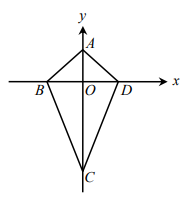
\includegraphics[scale=1]{./figure/2.png}
	\raggedleft %靠右對齊
\end{minipage}




\begin{tasks}(3)
	\task 此四數值中以$m_{\overline{AB}}$為最大
	\task 此四數值中以$m_{\overline{BC}}$為最小
	\task $m_{\overline{BC}} = -m_{\overline{CD}}$
	\task $m_{\overline{AB}} \times m_{\overline{BC}} = -1$
	\task $m_{\overline{CD}} + m_{\overline{DA}} > 0$
\end{tasks}

\begin{solution}~\\
	(B)(C)(E)
\end{solution}

%cas_8
\question
【中山】\\
\begin{minipage}[t]{0.7\linewidth}
	如圖,四邊形$ABCD$在桌標平面上,$\angle ADC = 90^{\circ}$,令$m_{AB}$,$m_{BC}$,$m_{CD}$,$m_{DA}$分別表直線$AB$,$BC$,$CD$,$DA$之斜率,請問以下哪些敘述成立($x$,$y$軸單位長為相等)
\end{minipage}
\hfill
\begin{minipage}[t]{0.3\linewidth}
	\vspace*{-0.3cm}
	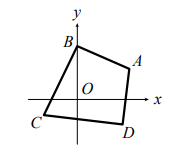
\includegraphics[scale=1]{./figure/3.png}
	\raggedleft %靠右對齊
\end{minipage}

\begin{tasks}(3)
	\task 此四數值中以$m_{BC}$為最大
	\task 此四數值中以$m_{AB}$為最小
	\task $m_{CD} = -m_{DA}= -1$
	\task $m_{CD} \times m_{BC} > -1$
	\task $m_{DA} + m_{CD} > 0$
\end{tasks}

\begin{solution}~\\
	(B)(C)(D)(E)
\end{solution}


%cas_9
\question
【南一中】\\
\begin{minipage}[t]{0.7\linewidth}
	觀察圖中線段的斜率,試問下列選項何者為真?
\end{minipage}
\hfill
\begin{minipage}[t]{0.3\linewidth}
	\vspace*{-0.3cm}
	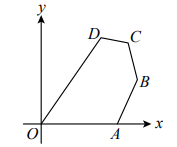
\includegraphics[scale=1]{./figure/4.png}
	\raggedleft %靠右對齊
\end{minipage}

\begin{tasks}(3)
	\task $\overline{OA}$的斜率最小
	\task $\overline{AB}$的斜率最大
	\task $\overline{BC}$的斜率最小
	\task $\overline{CD}$的斜率介於$0$,$1$之間
	\task $\overline{OD}$的斜率介在$1$,$2$之間。
\end{tasks}
\begin{solution}~\\
	(B)(C)(E)
\end{solution}


%cas_10
\question
【道明】\\
\begin{minipage}[t]{0.7\linewidth}
	右圖之$12$個點(左右、上下間格相同),則由這些點連成之直線共有\ul{50pt}種方向。
\end{minipage}
\hfill
\begin{minipage}[t]{0.3\linewidth}
	\vspace*{-0.3cm}
	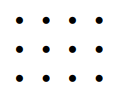
\includegraphics[scale=1]{./figure/5.png}
	\raggedleft %靠右對齊
\end{minipage}

\begin{solution}~\\
	12
\end{solution}


%cas_11
\question
【花蓮】\\
\begin{minipage}[t]{0.7\linewidth}
	途中是座標平面上的十六個點(左、右、上、下間格均相等),這些點中任意兩點連成直線不考慮無斜率的情形,則斜率最小者為下列哪一個數值?
\end{minipage}
\hfill
\begin{minipage}[t]{0.3\linewidth}
	\vspace*{-0.3cm}
	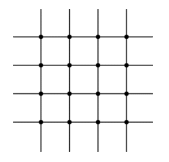
\includegraphics[scale=1]{./figure/6.png}
	\raggedleft %靠右對齊
\end{minipage}

\begin{tasks}(5)
	\task $-4$
	\task $-3$
	\task $-2$
	\task $-1$
	\task 以上皆非
\end{tasks}

\begin{solution}~\\
	(B)
\end{solution}

%cas_12
\question
【鳳山】\\
\begin{minipage}[t]{0.7\linewidth}
	如圖所示,直線$L$分別與$x$軸、$y$軸交於$A$、$B$,已知$C\left( 4,9 \right)$在$L$上,且$4\overline{AB}=\overline{BC}$,試問直線$L$之斜率為下列何值?
\end{minipage}
\hfill
\begin{minipage}[t]{0.3\linewidth}
	\vspace*{-0.3cm}
	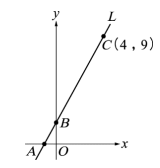
\includegraphics[scale=1]{./figure/7.png}
	\raggedleft %靠右對齊
\end{minipage}


\begin{tasks}(5)
	\task $\frac{1}{2}$
	\task $\frac{2}{3}$
	\task $1$
	\task $\frac{3}{2}$
	\task $\frac{9}{5}$
\end{tasks}
\begin{solution}~\\
	(E)
\end{solution}

%cas_13
\question
【附中】\\
\begin{minipage}[t]{0.7\linewidth}
	如圖,$\triangle OAB$與$\triangle OPQ$對應全等,若過$O$,$A$兩點的直線斜率為k,試問過$O$、$P$兩點的直線斜率為何?
\end{minipage}
\hfill
\begin{minipage}[t]{0.3\linewidth}
	\vspace*{-0.3cm}
	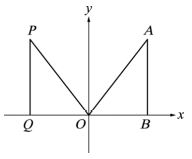
\includegraphics[scale=1]{./figure/8.png}
	\raggedleft %靠右對齊
\end{minipage}

\begin{tasks}(4)
	\task $\frac{1}{k}$
	\task $k$
	\task $-\frac{1}{k}$
	\task $-k$
\end{tasks}

\begin{solution}~\\
	(D)
\end{solution}

%cas_14
\question
【嘉女】\\
\begin{minipage}[t]{0.7\linewidth}
	座標平面上有一個正方形,其中有一邊所在的直線斜率為$5$,而此正方形兩對角線所在的直線斜率分別為$m_1$,$m_2$,且$m_1 < m_2$,則$m_1=$\ul{50pt}。
\end{minipage}
\hfill
\begin{minipage}[t]{0.3\linewidth}
	\vspace*{-0.3cm}
	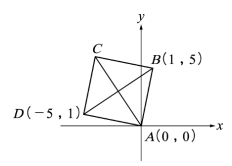
\includegraphics[scale=1]{./figure/9.png}
	\raggedleft %靠右對齊
\end{minipage}

\begin{solution}~\\
	$-\dfrac{3}{2}$
\end{solution}

%cas_15
\question
【明倫】\\
設$y = f(x)$為一線性函數通過兩點$A\left( -1,-1\right)$、$B\left( 2,5\right)$,則$\frac{f(4321)-f(1234)}{4321-1234} = $\ul{50pt}
\begin{solution}~\\
	$2$
\end{solution}


%cas_16
\question
【松山】\\
已知一次函數$f(x)$通過兩點$\left( -2,15\right)$與$\left( 4,6\right)$,則$f(2016)-f(2014)=$\ul{50pt}。
\begin{solution}~\\
	$-3$
\end{solution}

%cas_17
\question
【內湖】\\
已知一次函數$f(x)=ax+b$,每當$x$增加$2$單位時,其對應的函數值減少$6$單位,又已知$f(1)=5$,則下列哪些選項正確?

\begin{tasks}(1)
	\task $y=f(x)$之圖形斜率為$3$
	\task $y=f(x)$之圖形的$y$截距為$\left( 0,8\right)$
	\task $y=f(x)$之圖形不通過第三象限
	\task $y=f(x)$之圖形對於$x$軸的對稱圖形之方程式為$-y=ax+b$
	\task $y=f(x)$之圖形可由函數$y=g(x)=ax$的圖形向上平移$8$單位而得
\end{tasks}

\begin{solution}~\\
	(B)(C)(D)(E)
\end{solution}

%cas_18
\question
【明倫】\\
若$A\left( 3,-2\right)$、$B\left( 1,4\right)$、$C\left( k,1\right)$三點共線,則$k=$\ul{50pt}
\begin{solution}~\\
	$2$
\end{solution}

%cas_19
\question
【板中】\\
已知直線$y=ax+b$的圖形上$A\left( 2,-2\right($、$B\left(k+2,0\right)$、$C\left(k-8,-5\right)$三點,則序組$\left( a,b,k \right) =$\ul{50pt}。
\begin{solution}~\\
	$\left(  \dfrac{1}{2},-3,4  \right)$
\end{solution}

%cas_20
\question
【丹鳳】\\
今日環保局由報案專線接獲三位民眾投訴住家附近有工廠在偷排放濃硝酸,造成嚴重空汙。環
保局便立即指派欽欽、秀秀、惠惠三位稽查員前往稽查,若經查獲屬實者,環保局將依空氣汙
染防治法重罰$100$萬元罰鍰。已知欽欽從環保局出發,向北行駛$8$公里,再向西行駛$3$公里抵達第一位民眾投訴地點;秀秀從環保局出發,向南行駛$k$公里,再向東行駛$10$公里抵達第二
位民眾投訴地點;惠惠從環保局出發,向東行駛$4$公里,再向北行駛$k$公里抵達第三位民眾投
訴地點。若三個投訴地點位於同一直線上,則正數$k$之值為\ul{50pt}。
\begin{solution}~\\
	$\dfrac{12}{5}$
\end{solution}


%cas_21
\question
【成淵】\\
座標平面上有四點$A\left(-3,1\right)$、$B\left(3,2 \right)$、$C\left( k,5 \right)$、$D\left( -1,4\right)$,若直線$AB$垂直直線$CD$,則$k=$\ul{50pt}
\begin{solution}~\\
	$-\dfrac{7}{6}$
\end{solution}

%cas_22
\question
【明倫】\\
已知$A\left(3,-2\right)$、$B\left(-1,0 \right)$、$C\left( 2,k \right)$為$\triangle ABC $的三頂點且$ \angle A = 90^{\circ}$,求$k=$\ul{50pt}
\begin{solution}~\\
	$-4$
\end{solution}

%cas_23
\question
【竹北】\\
已知三點$A\left( 1,2\right($、$B\left( 3,6 \right)$、$C\left(4,k\right)$,$k\in \mathbb{R}$。若$\triangle ABC$為直角三角形,求$k$之值為\ul{50pt}
\begin{solution}~\\
	$\dfrac{1}{2}  \vee \dfrac{11}{2} \vee 3 \vee 5$
\end{solution}

%cas_24
\question
【大直】\\
平面上有$A\left(0,0\right)$、$B\left( 10,0\right)$、$C\left( k,4\right)$共三點,且$\triangle ABC$為直角三角形,選出$k$的解個數。
\begin{tasks}(5)
	\task $1$
	\task $2$
	\task $3$
	\task $4$
	\task 無限多解
\end{tasks}

\begin{solution}~\\
	(D)
\end{solution}


%cas_25
\question
【西松】\\
座標平面上,已知過點$P\left( 5,4\right)$做互相垂直的兩直線與$x$軸焦於兩點$A,B$,若$\overline{AB}=10$,且$A,B$的中點座標為$\left( t,0 \right)$,則$t=$\ul{50pt}
\begin{solution}~\\
	$2$或$8$
\end{solution}

%cas_26
\question
【中女中】\\
設$a,b$為實數,若點$\left( 3,2\right)$對直線$2x+3y+a=0$的垂足為$\left( b,-1 \right)$,則數對$\left( a,b\right) = $\ul{50pt}
\begin{solution}~\\
	$\left( 1,1 \right($
\end{solution}

%cas_27
\question
【建中】\\
平面上有一個等腰直角三角形,已知其三邊長的斜率分別為$m_1$、$m_2$、$m_3$,且$m_1>m_2>m_3$,請選出正確的選項。

\begin{tasks}(5)
	\task $m_1 > 0$
	\task $m_2 \leq 0$
	\task $m_3 < 0$
	\task $m_1 = -m_3$
	\task $m_1m_3=-1$
\end{tasks}

\begin{solution}~\\
	(A)(C)
\end{solution}


\subsubsection{直線方程式}

%linef_1
\question
【明倫】\\
設直線$L$的斜率為$3$,且在$x$軸的截距為$2$,求直線$L$的方程式為\ul{50pt}。
\begin{solution}~\\
	$y = 3x - 6$
\end{solution}

%linef_2
\question
【中女中】\\
設直線$L$通過兩點$\left( 3,2\right)$、$\left( 4,-1\right)$,則$L$的方程式為\ul{50pt}。
\begin{solution}~\\
	$3x + y - 11 = 0$
\end{solution}

%linef_3
\question
【三民】\\
設直線$L$通過點$\left( 4,1\right)$ 且$y$截距為$5$,求$L$的直線方程式為\ul{50pt}。
\begin{solution}~\\
	$x + y = 5$
\end{solution}

%linef_4
\question
【屏中】\\
$A\left( -2,3\right)$、$B\left( 1,9\right)$,求過點$\left( 1,2\right)$且平行$\overline{AB}$的直線方程式為\ul{50pt}。
\begin{solution}~\\
	$2x - y = 0$
\end{solution}

%linef_5
\question
【豐原】\\
過$x+2y=3$與$2x-y=1$之交點且與$3x-y+6=0$平行之線性方程式為\ul{50pt}。
\begin{solution}~\\
	$3x - y - 2 = 0$
\end{solution}

%linef_6
\question
【屏中】\\
一直線$L_1$過$\left( 1,3\right($、$\left( 2,-1\right($兩點,另一直線$L_2$過$\left( 3,-2  \right)$且與$L_1$垂直,則直線$L_2$的方程式為\ul{50pt}
\begin{solution}~\\
	$y + 2 = \frac{1}{4} \left( x-3 \right)$
\end{solution}

%linef_7
\question
【延平】\\
設直線$L$過$17x+11y+5=0$與$13x+23y+9=0$的交點,且$L$與直線$x-3y+2=0$垂直,則$L$的方程式為\ul{50pt}
\begin{solution}~\\
	$x + y = - \frac{17}{31}$
\end{solution}

%linef_8
\question
【華江】\\
$\triangle ABC$中,已知$A\left( 2,0\right($,且$D\left( 3,4\right)$、$E\left( 6,5\right)$分別為$\overline{AB}$與$\overline{BC}$之中點,若直線$AC$的方程式為$ax-by-2=0$其中$a,b$均為整數,則數對$\left( a,b \right)=$\ul{50pt}。
\begin{solution}~\\
	$\left( 1,3 \right)$
\end{solution}

%linef_9
\question
【三民】\\
\begin{minipage}[t]{0.7\linewidth}
	如圖,$O$為座標原點,直線$L$與$x$軸、$y$軸分別交於$A$與$B$兩點,已知$\overline{OA}=2\overline{OB}$且直線$L$過點$C\left( 1,1\right)$,則$L$的方程式為\ul{50pt}
\end{minipage}
\hfill
\begin{minipage}[t]{0.3\linewidth}
	\vspace*{-0.3cm}
	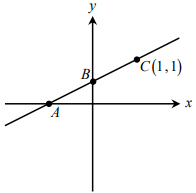
\includegraphics[scale=1]{./figure/10.png}
	\raggedleft %靠右對齊
\end{minipage}

\begin{solution}~\\
	$x-2y+1=0$
\end{solution}

%linef_10
\question
【成淵】\\
請選出斜率最小的直線:
\begin{tasks}(3)
	\task $2x+y+1=0$
	\task $3x-4y+5=0$
	\task $y-3=8\left( x+1\right)$
	\task $y=5x-7$
	\task $\frac{x}{2}+\frac{y}{3}=1$
\end{tasks}
\begin{solution}~\\
	(A)
\end{solution}

%linef_11
\question
【98學測】\\
\begin{minipage}[t]{0.7\linewidth}
	坐標平面上四條直線$L_1$、$L_2$、$L_3$、$L_4$與$x$軸、$y$軸及直線$y=x$的相關位置如圖所示,其中$L_1$與$L_3$垂直,而$L_3$與$L_4$平行。設$L_1$、$L_2$、$L_3$、$L_4$的方程式分別為$y=m_1x$,$y=m_2x$,$y=m_3x$以及$y=m_4x+c$。試問下列哪些選項是正確的?
\end{minipage}
\hfill
\begin{minipage}[t]{0.3\linewidth}
	\vspace*{-0.3cm}
	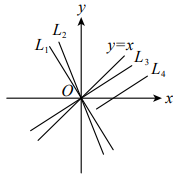
\includegraphics[scale=1]{./figure/11.png}
	\raggedleft %靠右對齊
\end{minipage}


\begin{tasks}(3)
	\tasks $m_3 > m_2 > m_1$
	\tasks $m_1 \cdot m_4 = -1$
	\tasks $m_1 < -1$
	\tasks $m_2 \cdot m_3 < -1$
	\tasks $c > 0$
\end{tasks}

\begin{solution}~\\
	(B)(C)(D)
\end{solution}

%linef_12
\question
【松山】\\
\begin{minipage}[t]{0.7\linewidth}
	如圖,三直線的方程式依次為$L_1:y=a_1x+b_1$,$L_2:y=a_2x+b_2$,$L_3:y=a_3x+b_3$,下列選項何者正確?
\end{minipage}
\hfill
\begin{minipage}[t]{0.3\linewidth}
	\vspace*{-0.3cm}
	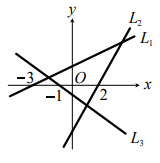
\includegraphics[scale=1]{./figure/12.png}
	\raggedleft %靠右對齊
\end{minipage}


\begin{tasks}(5)
	\task $a_1 > a_2$
	\task $b_2 > b_3$
	\task $a_1b_2 > a_2b_2$
	\task $2a_3 > b_3$
	\task $a_2 + b_2 < 0$。
\end{tasks}
\begin{solution}~\\
	(C)(E)
\end{solution}

%linef_13
\question
【中山】\\
\begin{minipage}[t]{0.7\linewidth}
	如圖,$L_1:y=ax+b$,$L_2:y=cx+d$,$L_3:y=ex+f$,下列各數哪一個最小?
\end{minipage}
\hfill
\begin{minipage}[t]{0.3\linewidth}
	\vspace*{-0.3cm}
	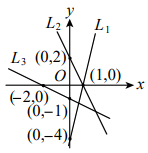
\includegraphics[scale=1]{./figure/13.png}
	\raggedleft %靠右對齊
\end{minipage}

\begin{tasks}(5)
	\task $a$
	\task $b$
	\task $c$
	\task $d$
	\task $e$
\end{tasks}
\begin{solution}~\\
	(B)
\end{solution}

%linef_14
\question
【雄中】\\
\begin{minipage}[t]{0.7\linewidth}
	如圖,,三直線$L_1:y=m_1x+b_1$,$L_2:y=m_2x+b_2$,$L_3:y=m_3x+b_3$,下列有關$m_1$、$m_2$、$m_3$、$b_1$、$b_2$、$b_3$之選項,何者正確?
\end{minipage}
\hfill
\begin{minipage}[t]{0.3\linewidth}
	\vspace*{-0.3cm}
	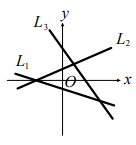
\includegraphics[scale=1]{./figure/14.png}
	\raggedleft %靠右對齊
\end{minipage}

\begin{tasks}(3)
	\task $m_3<m_1<m_2$
	\task $m_1<m_2<m_3$
	\task $b_2>b_3>b_1$
	\task $b_3>b_2>b_1$
	\task $b_1>b_2>b_3$
\end{tasks}

\begin{solution}~\\
	(A)(D)
\end{solution}


%linef_15
\question
【景美】\\
(1)不論$m$為任何實數,直線$L:y=mx-m+3$恆過定點$P$,求$P$座標為\ul{50pt}。\\
(2)承(1),已知$A\left( -1,-3\right)$、$B\left( 4,2\right)$,若$L$與$\overline{AB}$相交,求$m$的範圍為\ul{50pt}。

\begin{solution}~\\
	(1)$ \left(  1,3 \right)$(2)$m \leq - \frac{1}{3} \vee m \geq 3$
\end{solution}

%linef_16
\question
【中女中】\\
已知直線$L:mx-y+3-m=0$與兩點$A\left( -2,-3\right)$、$B\left( 3,2\right)$,若$L$與$\overline{AB}$不相交,試求實數$m$的範圍為\ul{50pt}。
\begin{solution}~\\
	$-\frac{1}{2} < m < 2$
\end{solution}

%linef_17
\question
【竹北】\\
設$A\left( 1,5\right)$、$B\left( 4,1\right)$、$C\left( 2,-1\right)$,直線$L:mx-2m-y+6=0$,若直線$L$與$\triangle ABC$有交點,求$m$的最大可能範圍為\ul{50pt}。
\begin{solution}~\\
		$m \leq - \frac{5}{2} \vee m \geq 1$
\end{solution}

%linef_18
\question
【屏女】\\
$\triangle ABC$三邊所在的直線為$2x+y-3=0$、$y=0$、$x-y=0$,若直線$y=mx+3$與$\triangle ABC$相交,則$m$可能為下列何數?

\begin{tasks}(5)
	\task $-\frac{1}{3}$
	\task $ -5$
	\task $-2$
	\task $\frac{5}{2}$
	\task $1$
\end{tasks}
\begin{solution}~\\
	(B)(C)
\end{solution}

%linef_19
\question
【中崙】\\
令$A\left( 1,0\right)$、$B\left( 1,1\right)$、$\left( -1,1\right)$、$D\left( -1,0\right)$,若直線$y=mx+3$恆與長方形$ABCD$有交點,則$m$的值可能為?

\begin{tasks}(5)
	\task $0$
	\task $1$
	\task $2$
	\task $-3$
	\task $-4$
\end{tasks}


\begin{solution}~\\
	(C)(D)(E)
\end{solution}

%linef_20
\question
【華江】\\
座標平面中,設$A\left( -5,0\right)$與$B\left( -2,3\right)$,若直線$L:3x-4y+k=0$與$\overline{AB}$相交,則實數$k$的範圍是\ul{50pt}。

\begin{solution}~\\
	$15 \leq k \leq 18$
\end{solution}

%linef_21
\question
【三民】\\
座標平面三點$A\left( 3,4\right)$、$B\left( -2,-5\right)$、$C\left( 7,0\right)$,過$B$點將$\triangle ABC$的面積等分的直線方程式為\ul{50pt}。

\begin{solution}~\\
	$x-y=3$
\end{solution}

%linef_22
\question
【成功】\\
某直線通過點$\left( 7,4\right)$,且將平行四邊形$ABCD$之面積平分,若$A\left( 1,1\right)$、$B\left( 3,4\right)$、$C\left( 9,5\right)$、$D\left( 7,2\right)$為平行四邊形$ABCD$的四個頂點,求直線方程式為\ul{50pt}。
\begin{solution}~\\
	$x-2y+1=0$
\end{solution}

%linef_23
\question
【建中】\\
已知點$A\left( 9,-2\right)$,點$B\left( -1,8\right)$,直線$L:x-2y+7=0$,若$Q$為$L$上使$\angle AQB$為直角的點,求$Q$點座標為\ul{50pt}。
\begin{solution}~\\
	$\left( -3,2 \right) \vee \left( 9,8 \right)$
\end{solution}

%linef_24
\question
【板中】\\
已知$A\left( 4,6\right)$、$B\left( 8,2\right)$、$C\left( 5,-7\right)$,$\overline{AB}$邊上的高所在的直線方程式為\ul{50pt}。
\begin{solution}~\\
	$x-y-12=0$
\end{solution}

%linef_25
\question
【北一】\\
$A\left( 1,2\right)$、$B\left( 5,-2\right)$為座標平面上的兩點,則$\overline{AB}$之中垂線方程式為\ul{50pt}。

\begin{solution}~\\
	$x-y=3$
\end{solution}

%linef_26
\question
【前鎮】\\
已知平面上$A\left( 1,3\right)$、$B\left( -2,2\right)$兩點,若$P$點在$x$軸上,且$\overline{PA}=\overline{PB}$,則$P$點座標為\ul{50pt}。

\begin{solution}~\\
	$\left( \frac{1}{3} ,0\right)$
\end{solution}

%linef_27
\question
【松山】\\
鳶形$ABCD$(其中$\overline{AB}=\overline{AD}$、$\overline{CB}=\overline{CD}$),已知$A\left( 2,-1\right)$、$B\left( 2,1\right)$、$C\left( -2,3\right)$,求$D$點座標為\ul{50pt}
\begin{solution}~\\
	$\left( 0,-1 \right)$
\end{solution}

%linef_28
\question
【景美】\\
已知平行四邊形的兩邊所在直線方程式為$2x+y=18$及$x-y=-6$,且一頂點為$\left( 3,-6\right)$,求此平行四邊形在第二象限上的頂點座標為\ul{50pt},
\begin{solution}~\\
	$\left( -2,4 \right)$
\end{solution}

%linef_29
\question
【新店】\\
一平行四邊形兩邊分別在直線$2x-y+2=0$及$x+3y-6=0$上,其中一頂點為$\left( 2,-1\right)$,則此平行四邊形之周長為\ul{50pt}。
\begin{solution}~\\
	$2\sqrt{5}+2\sqrt{10}$
\end{solution}

%linef_30
\question
【中女中】\\
一直線$L$通過點$\left( -3,2\right)$,若$L$的$x$截距與$y$截距恰為相反數且皆為非0實數,則直線$L$的方程式為\ul{50pt}
\begin{solution}~\\
	$x-y+5=0$
\end{solution}


%linef_31
\question
【基中】\\
若有一直線在坐標軸上之$x$截距與$y$截距相等且通點$\left( -4,2\right)$,則直線方程式為\ul{50pt}。
\begin{solution}~\\
	$x+2y=0 \vee x+y+2=0$
\end{solution}

%linef_32
\question
【高師】\\
設直線$L$通過點$\left( -2,3\right)$且與$x$軸、$y$軸截距的絕對值相等,則$L$之方程式為\ul{50pt}。
\begin{solution}~\\
	$3x+2y=0 \vee x+y = 1 \vee x - y = -5$
\end{solution}

%linef_33
\question
【附中】\\
求截距和為$3$與$2x-y+4=0$垂直的直線方程式為\ul{50pt}。
\begin{solution}~\\
	$x+2y = 2$
\end{solution}

%linef_34
\question
【雄女】\\
設一直線$L$與$4x+5y+7=0$垂直,且$L$的兩截距和為$4$,若$L$的方程式為$x+by+c=0$,則數對$\left( b,c\right)=$\ul{50pt}。
\begin{solution}~\\
	$\left( -\frac{4}{5},16\right)$
\end{solution}

%linef_35
\question
【延平】\\
若直線$L$通過點$\left( 9,8\right)$,且直線$L$與兩座標軸所圍成的區域面積為$3$,則直線$L$的直線方程式為\ul{50pt}。
\begin{solution}~\\
	$32x-27y-72=0 \vee 2x-3y+6=0 $
\end{solution}

%linef_36
\question
【松山】\\
一直線在第三象限內與兩軸所圍成之三角形面積為$6$,已知此直線的斜率為$-\frac{1}{3}$,求此直線方程式為\ul{50pt}。
\begin{solution}~\\
	$x+3y+6=0$
\end{solution}

%linef_37
\question
【北一】\\
設直線$L$的斜率是$\frac{3}{2}$,且與兩座標軸所圍成的三角形面積為$12$,求$L$的方程式為\ul{50pt}。
\begin{solution}~\\
	$3x-2y=12 \vee 3x-2y = -12$
\end{solution}

%linef_38
\question
【中女中】\\
設直線$L$過$\left( 3,-5\right)$且與兩座標軸於第四象限所形成的三角面積為最小時,試求:\\
(1)直線$L$的方程式為\ul{50pt}。(請化為$ax+by+c=0$的形式)\\
(2)此最小的三角形面積為\ul{50pt}\\
\begin{solution}~\\
	(1)$5x-3y = 30$(2)$30$
\end{solution}

%linef_39
\question
【建中】\\
平面上有一定點$P\left( 1,1\right)$,一直線$L$過$P$點且與$x$軸、$y$軸分別交流於$A$、$B$兩點($L$不經過原點),原點為$O$,則此三點所形成的三角形$OAB$,\\
(1)求在第一象限所圍成的三角形$OAB$的面積的最小值$t=$\ul{50pt}及當時直線$L$的方程式為\ul{50pt}。\\
(2)若三角形$OAB$的面積為$4$,則滿足此種條件之直線$L$的方程式為\ul{50pt}
\begin{solution}~\\
	(1)$2$;$x+y-2=0$(2)$\left( 2 + \sqrt{2}\right) x + \left( 2-\sqrt{2}\right) y -4=0$或$\left( 2 - \sqrt{2}\right) x + \left( 2+\sqrt{2}\right) y -4=0$或$\left( -2 + \sqrt{6}\right) x + \left( -2 -\sqrt{6}\right) y +4=0$或$\left( -2 - \sqrt{6}\right) x + \left( -2 +\sqrt{6}\right) y +4=0$
\end{solution}

\subsubsection{三角形的心}

%trih_1
\question
【華江】\\
$\triangle ABC$之三頂點$A\left( 4,4\right)$、$\left( 0,-4\right)$、$C\left( 6,2\right)$,則下列何者正確?

\begin{tasks}(3)
	\task $\overline{AB}$的垂直平分線方程式為$x+2y-2=0$
	\task $\overline{AC}$的垂直平分線方程式為$x-y-2=0$
	\task $\triangle ABC$的外心座標為$\left( 2,0\right)$
	\task $\triangle ABC$為直角三角形
	\task $\triangle ABC$的面積為$12$
\end{tasks}
\begin{solution}~\\
	(A)(B)(C)(D)(E)
\end{solution}

%trih_2
\question
【陽明】\\
已知有$A$、$B$、$C$三所學校,在某份都市計畫圖中,顯示其座標分為$A\left( 0,2\right)$、$B\left( 1,1\right)$、$C\left( 2,-2\right)$。若都市計畫委員想蓋一座圖書館,使他與$A$、$B$、$C$三所學校的距離都相等,試問該圖書館在此地圖中的座標為\ul{50pt}。
\begin{solution}~\\
	$\left( -3,-2\right)$
\end{solution}

%trih_3
\question
【延平】\\
設$A\left( -1,5\right)$,$B\left( 7,1\right)$,$C\left( 5,-3\right)$,\\
(1)求$\triangle ABC$的外心座標為\ul{50pt}。(外心為三中垂線的交點)
(2)求$\triangle ABC$的垂心座標為\ul{50pt}。(垂心為三高的交點)
\begin{solution}~\\
	(1) $\left( 2,1\right)$(2)$\left( 7,1\right)$
\end{solution}

%trih_4
\question
【雄中】\\
$A\left( 1,-1\right)$,$B\left( -4,1\right)$,$C\left( 4,3\right)$,求$\triangle ABC$之外心$O$為\ul{50pt},垂心$H$為\ul{50pt},重心$G$為\ul{50pt},並檢驗三點是否共線?\ul{50pt}。
\begin{solution}~\\
	$\left( -\frac{7}{26} ,\frac{40}{13} \right)$ ,$\left( \frac{20}{13},-\frac{41}{13} \right)$,$\left( \frac{1}{3},1 \right)$,是
\end{solution}

%trih_5
\question
【雄中】\\
平面座標系上,點$A\left( 2,-1\right)$、$B\left( 6,-3\right)$。若$\triangle ABC$的重心座標為$\left( \frac{7}{3},\frac{-14}{3}\right)$,試求$\triangle ABC$的垂心座標為\ul{50pt}。
\begin{solution}~\\
	$\left( 3,-2 \right)$
\end{solution}

%trih_6
\question
【北一】\\
在$\triangle ABC$中,$B\left( 2,3\right)$,$C\left( 8,2\right)$,垂心$H\left( \frac{34}{7},\frac{36}{7}\right)$,則頂點$A$的座標為\ul{50pt}。
\begin{solution}~\\
	$\left( 5,6\right)$
\end{solution}

%trih_7
\question
【三民】\\
設$A\left( -1,-5\right)$、$B\left( 7,1\right)$、$C\left( 5,-3\right)$。外心$O$為三中垂線的交點,垂心$H$為三高的交點,求$OH$的直線方程式為\ul{50pt}。
\begin{solution}~\\
	$y-1=0$
\end{solution}

%trih_8
\question
【中正】\\
已知$A\left( 3,2\right)$、$B\left( 9,2\right)$、$C\left( 4,5\right)$,設$\triangle  ABC$的重心為$G$,外心為$O$,$G$和$O$兩點的連線稱為尤拉線,求尤拉線的直線方程式為\ul{50pt}。
\begin{solution}~\\
	$3x+6y=34$
\end{solution}


\end{questions}

\end{document}
